\documentclass[12pt]{article}

\usepackage[utf8]{inputenc}
\usepackage[T1]{fontenc}
\usepackage[francais]{babel}
\usepackage{multirow}
\usepackage{array}
\usepackage{color}
\usepackage{stmaryrd}
\usepackage{fancyhdr}
\usepackage{afterpage}
\usepackage{fullpage}
\usepackage{geometry}
\usepackage{setspace}
\usepackage{enumitem}
\usepackage{hyperref}
\usepackage{graphicx}
\usepackage{titling}
\usepackage{wrapfig}
\usepackage{float}
\usepackage{placeins}
\usepackage{caption}

% Enlève les contours des liens
\hypersetup{
    linkbordercolor={1 1 1},
    citebordercolor={1 1 1},
    urlbordercolor={1 1 1},
    colorlinks=true,
    linkcolor=black,
    urlcolor=blue
}
\PassOptionsToPackage{hyphens}{url}\usepackage{hyperref}

\pagestyle{fancy}
\setlength{\headheight}{12pt}
\fancyhf{}
\fancyhead[L]{Benoit HOUDAYER, Anthony RUHIER}
\fancyhead[R]{Dawwyd -- Dossier Fonctionnel}
\geometry{headsep=5ex}

\graphicspath{{images/}}


\title{\vspace{-1cm}\textbf{%
    SI75 -- Logiciel de Commande Vocale \vspace{0.5cm}
    \protect
\includegraphics[width=4cm]{logo.jpg}\\[0.5em]
    Dossier Technique}}

\author{Benoit HOUDAYER \\ \href{mailto:benoit.houdayer@utbm.fr}{benoit.houdayer@utbm.fr}
\and Anthony RUHIER \\ \href{mailto:anthony.ruhier@utbm.fr}{anthony.ruhier@utbm.fr}}

\date{29 janvier 2016}

\postauthor{\end{tabular}\vspace{0.6cm} \par Université de Technologie de Belfort-Montbéliard\end{center}}

\begin{document}
    \maketitle
    \thispagestyle{empty}
    \tableofcontents
    \listoffigures

    \section*{Historique des modifications}

    \begin{table}[H]
    \centering

    \begin{tabular}{|l|l|l|l|}
        \hline
        version & date & auteur & modification \\
        \hline
        0.1 & 28 janvier 2016 & BHD & création du document \\
        0.2.6 & 28 janvier 2016 & ARH & ajout des diagrammes UML \\
        \hline
    \end{tabular}
    \end{table}

    \afterpage{\cfoot{\thepage}}
    \newpage

    \section{Solutions Utilisées}
	    \subsection{Système d'exploitation}
	    \paragraph{}
        Dawwyd est prévu pour fonctionner dans un environnement Linux. Les
        raisons de ce choix sont :
	    \begin{itemize}
	    	\item L'expérience Linux de l'équipe de développement
            \item La grande variété de machines supportant le système
                d'exploitation Linux
	    \end{itemize}

	    \paragraph{}

	    Le support de plusieurs types de machines est un point important pour Dawwyd; comme il ne nécessite pas d'interface graphique, on peut envisager d'utiliser l'application aussi bien sur une station de travail classique (ordinateur de bureau ou portable) que sur un serveur domestique, diffusant de la musique (par exemple, une instance de \label{mpd} MPD\footnote{\url{http://www.musicpd.org/}} sur une architecture ARM ou Spotify sur X86)
	    
	    \subsection{Reconnaissance et Synthèse Vocale avec Jasper}
        \paragraph{}
        Jasper\footnote{\url{https://jasperproject.github.io/}} est un
        framework facilitant la reconnaissance vocale (Speech To Text : STT) et
        la synthèse vocale (Text To Speech : TTS).

	    \paragraph{}
        Le rôle de Jasper est de faciliter l'utilisation de moteurs de
        reconnaissance vocale divers, donnant plus de souplesse au projet. Les
        moteurs supportés et envisageables pour Dawwyd sont :

	    \begin{description}

	    	\item[PocketSphinx :] moteur open-source de reconnaissance vocale hors ligne. Idéalement, ce moteur est utilisé pour permettre l'utilisation de Dawwyd hors-ligne et préserver la vie privée de l'utilisateur.
	    	\item[Google STT :] moteur de reconnaissance vocale de Google. Il est plus précis que PocketSphinx mais nécessite une connexion internet pour fonctionner. En effet, la reconnaissance est effectuée par les serveurs de Google à partir d'un fichier audio qui leur est envoyé.
	    	\item[Wit.ai :] comme pour Google STT, ce moteur nécessite une connexion à internet. Il peut toutefois être une alternative intéressante.

	    \end{description}

	    \paragraph{}

	    Jasper supporte également de nombreuses solutions de synthèse vocale. Le moteur de synthèse vocale n'est pas crucial au fonctionnement de l'application, aussi, nous testeront l'application avec le moteur Espeak\footnote{\url{http://espeak.sourceforge.net/}} exclusivement.
    
        \subsection{Langage de Programmation}

        Le langage de programmation retenu pour ce projet est Python.
                \begin{wrapfigure}{R}{0cm}
                	\centering
                	\raisebox{0pt}[\dimexpr\height-2\baselineskip\relax]{%
                        
\includegraphics[width=2cm]{logo-python}%
                    }
                	\caption[Logo de Python]{}
                \end{wrapfigure}

        \paragraph{}
        Python est un langage de script qui permet une très grande souplesse et
        offre des facilités de développement. C'est un langage très répandu sur
        les OS de type Linux, supportant une variété d'architectures.

        \paragraph{}
        Le choix du langage est motivé par sa souplesse et par le fait que
        Jasper propose une API dans ce langage.

	\section{Implémentation}

	\FloatBarrier
		
		L'implémentation de Dawwyd se décompose entre la configuration et l'adaptation de Jasper, et l'implémentation de plugins. Jasper dispose d'une interface simple d'utilisation pour implémenter des plugins, que nous allons présenter rapidement. Les détails sont disponibles dans la documentation de Jasper\footnote{\url{https://jasperproject.github.io/documentation/api/standard/}}.
			
		\subsection{Interface Entre les Plugins et Jasper}
		Les plugins implémentés doivent hériter de la classe abstraite SpeechHandlerPlugin (cf figure \ref{classes}) pour pouvoir être appelés par Jasper. Les méthodes à implémenter sont :
		\begin{description}
			\item[handle(text, mic, profile) : ] Cette méthode a pour paramètres le texte transcrit et le profil de l'utilisateur (comprenant son nom). Elle peut ensuite l'objet mic pour envoyer une réponse directement à l'utilisateur sous forme de synthèse vocale.
			
			\item[is\_valid(text) : ] Cette méthode permet à Jasper de tester la compatibilité du texte avec le plugin avant d'appeler la méthode handle().
			
			\item[get\_priority() : ] Cette méthode retourne la priorité du plugin sous forme d'un entier. La priorité détermine l'ordre dans lequel les méthodes is\_valid() de plugins seront testées par Jasper.
		\end{description}
		
		\paragraph{}
		L'appel d'un plugin (cf figure \ref{séquence}) étant géré par Jasper, celui-ci n'est instancié que lorsqu'une commande est émise par l'utilisateur (1). Jasper teste chaque plugin dans l'ordre des priorités grâce à leur méthode is\_valid() (2). Si le plugin retourne false, Jasper teste le plugin suivant. Sinon (3) Jasper envoie le texte de la commande utilisateur au plugin via la méthode handle().
		
		\paragraph{}
		La réponse (5) est générée par le plugin, puis envoyée au moteur de synthèse vocale via la méthode micro.say() .
		
		\begin{figure}
			\centering
				\makebox[\textwidth]{%
				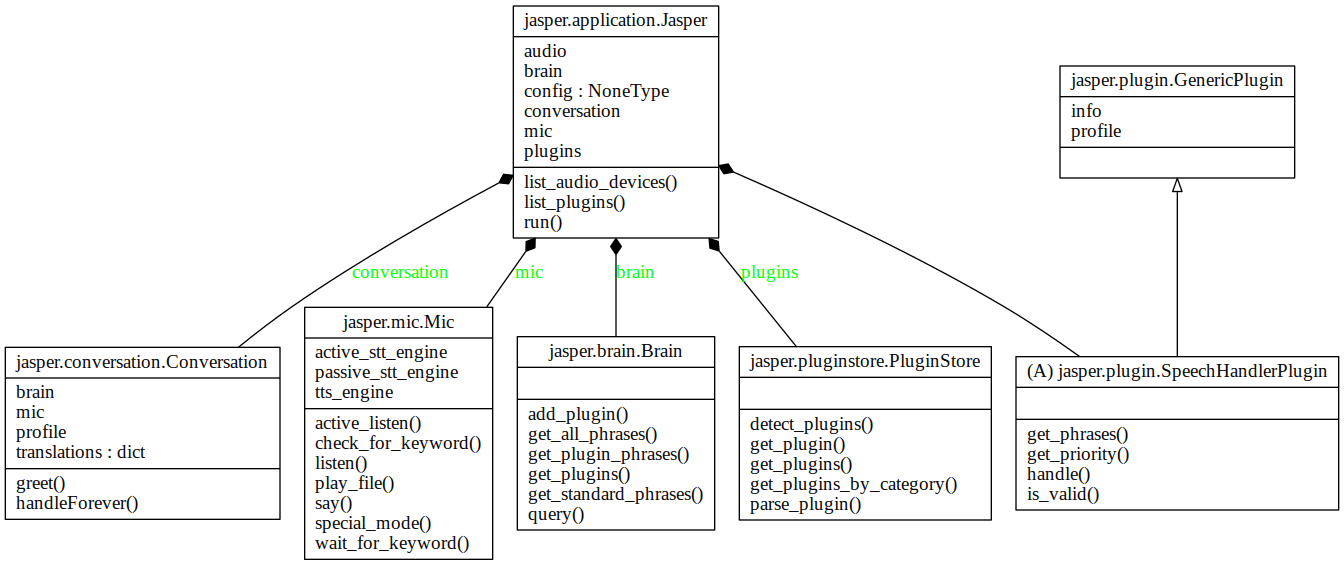
\includegraphics[width=19cm]{classes}%
			}
			\caption{\label{classes} Classes principales de Jasper}
		\end{figure}
	
		\begin{figure}
			\centering
				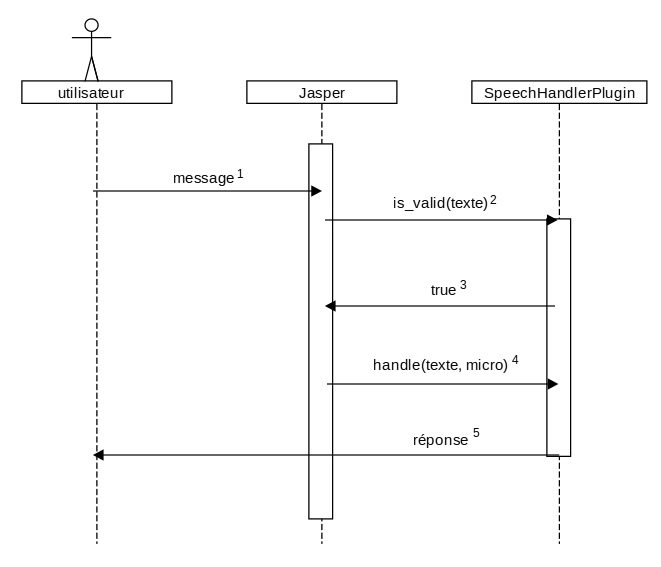
\includegraphics[width=\textwidth]{sequence}
				\caption{\label{séquence} Déroulement de l'Interprétation d'une Commande}
		\end{figure}

		\subsection{Précisions sur les Plugins}
		Les plugins seront implémentés suivant le temps restant au projet. Ils sont présentés ici par ordre de priorité.
		
		\subsubsection{Contrôle du lecteur audio}
		Le plugin de contrôle du lecteur audio est conçu pour contrôler uniquement le lecteur audio MPD\footnote{cf page \pageref{mpd}}. Toutefois, il peut être interfacé avec le logiciel Mopidy\footnote{\url{https://www.mopidy.com/}} pour supporter d'autres lecteurs audio, comme Spotify.
		
		\subsubsection{Contrôle du Navigateur}
		Le contrôle du navigateur consiste uniquement à ouvrir une nouvelle page dans le navigateur préféré de l'utilisateur; le plugin utilisera la commande système xdg-open pour choisir le bon navigateur.
		
		\paragraph{}
		L'utilisateur devra désigner une page par un alias pour qu'elle soit reconnue par Jasper. Les alias seront définis dans le fichier de configuration du plugin.
		
		\subsubsection{Actualités et Météo}
		Les plugins de récupération des Actualités et de la Météo utiliseront respectivement les API de Google News et de Yahoo pour récupérer les informations, avant de les restituer sous forme de synthèse vocale.

		\subsection{Conventions}
		Le développement doit se faire autant que possible en suivant les recommandations de la PEP~0008\footnote{\url{https://www.python.org/dev/peps/pep-0008/}}.

\end{document}
